\documentclass[10pt,twocolumn]{article}
\usepackage[margin=0.72in]{geometry}
\usepackage[T1]{fontenc}
\usepackage{amsmath,amssymb,booktabs,tabularx,array}
\usepackage{enumitem,graphicx,pgfplots,balance}
\usepackage[font=small,labelfont=bf]{caption}
\captionsetup[table]{skip=5pt}
\captionsetup[figure]{skip=6pt}
\pgfplotsset{compat=1.17}
\usepackage{hyperref}
\hypersetup{colorlinks=true,allcolors=black}
\urlstyle{same}
\setlength{\columnsep}{0.24in}
\setlength{\parindent}{1em}
\setlength{\parskip}{0.15em}
\setlength{\emergencystretch}{1.5em}
\setlength{\textfloatsep}{12pt plus 2pt minus 2pt}
\title{A Unified Study of Influence Maximization in Social Networks:\\
HIM, DeepSN, and GBIM}
\author{Course Project Final Report\\
Liu (HIM),\ Li Zixi (DeepSN),\ Jiang (GBIM)\\
Report assembled: 30 October 2026}
\date{}

\begin{document}
\maketitle

\begin{abstract}
We study influence maximization through three complementary methods: hyperbolic influence estimation (HIM), sheaf-neural diffusion estimation (DeepSN), and graph Bayesian optimization for multiplex interventions (GBIM). This report consolidates the team records and adds an audited HIM reproduction and selector-extension study. Nine new HIM training runs cover Cora-ML, Power Grid, and Facebook under fixed author-code WIC settings; three earlier Ciao models provide a real-topology, synthetic-diffusion extension. A neighborhood-overlap modification, ASW-J, does not yield stable gains. A second extension, HIM-C, combines a fixed HIM prior with global cumulative one-hop coverage selection. On a new evaluation stream, its average coverage exceeds ASW on Power Grid, Facebook, and Ciao, with unadjusted across-model intervals above zero, but not on Cora-ML. A coverage-only control shows that the current HIM prior does not provide stable additional benefit. The central finding is therefore a conditional improvement in seed selection, with explicit limits on attribution and generalization. DeepSN's recorded native and shared-Ciao results supply a complementary diffusion-model perspective; GBIM's user--information action space requires a separate comparison boundary. We do not report a universal three-way ranking or claim to reproduce every experiment in the original HIM paper.
\end{abstract}

\section{Problem and Project Scope}
We select the project theme of social-network transmission analysis, with influence maximization as the central task. Given a graph $G=(V,E)$, a diffusion process $\mathcal{M}$, and a budget $k$, the goal is to choose an initial seed set:
\begin{equation}
\begin{aligned}
S^*&\in\arg\max_{S\subseteq V,\ |S|\leq k}\sigma_{\mathcal M}(S),\\
\sigma_{\mathcal M}(S)&=\mathbb E[|A_{\mathcal M}(S)|].
\end{aligned}
\end{equation}
where $A_{\mathcal{M}}(S)$ is the set eventually activated from $S$. The practical difficulty is that the diffusion rules, edge probabilities, observed histories, and even the meaning of a ``seed'' differ across methods. Selecting high-degree users alone does not solve the set problem: two individually strong users may reach much of the same audience.

Our overall question is: \emph{How do graph-based influence methods use structural, propagation, and user--item evidence to select effective interventions under a limited budget?} The primary dataset is the Ciao review/trust network. The methods are linked through one data pipeline and a staged experiment: first compare user-level seed selection under one fixed propagation evaluator; then test whether item-aware user--item actions improve reach on the same users and trust graph. This preserves a common question without pretending the original objectives are interchangeable. DeepSN's native authors' protocol uses SIS on Jazz, whereas the shared Ciao contract uses weighted independent cascade (WIC). Those two numbers answer different questions and must never be pooled. Our contributions are an auditable reproduction pipeline, controlled selector extensions, and an empirical analysis of when geometric influence scores help or fail. We keep information assumptions and objective differences explicit.

\section{Related Methods and Their Connection}
Classical influence maximization maximizes expected spread under an explicit diffusion oracle. Under standard assumptions, the spread objective is monotone and submodular, allowing greedy selection to obtain a $1-1/e$ approximation with an exact marginal-gain oracle \cite{kempe}. Contact-process (SIS) dynamics allow recovered nodes to become susceptible again, so a reported ``infected share'' need not correspond to an absorbing activated set \cite{pastor}. The methods assigned in this project move beyond a single greedy oracle:
\begin{itemize}[leftmargin=1.2em,itemsep=0.1em]
  \item \textbf{HIM} learns one user embedding from social edges and observed propagation activations. Its Lorentzian distance to the origin estimates individual influence strength; its adaptive sliding window (ASW) adjusts scores of nearby candidate neighbors to reduce likely overlap \cite{him}.
  \item \textbf{DeepSN} treats influence as a learned map from a seed indicator to an activation pattern. Restriction maps of a cellular sheaf allow neighbor-to-neighbor influence to be heterogeneous rather than a shared scalar weight \cite{hansen,bodnar,deepsn}. Seed assignment then uses community-proportional budget allocation rather than a single radial score.
  \item \textbf{GBIM} uses graph Bayesian optimization for multiplex influence maximization. Its native decision is over user--information pairs on user and item-related graphs, not simply a set of users \cite{gbim}.
\end{itemize}
DeepIM offers a related seed-set representation-learning approach, but is not one of the three assigned implementations in this project \cite{deepim}. The methods can be presented as complementary views of a single pipeline: observed graph and interaction data; representation or surrogate learning; seed/action selection; and independent cascade evaluation. HIM emphasizes geometric influence ranking plus overlap correction, DeepSN emphasizes a richer neural model of propagation, and GBIM emphasizes sample-efficient optimization in a multiplex action space. They should not be combined into an ensemble merely because they share the phrase ``influence maximization.''

\begin{table*}[t]
\centering\small
\caption{Method roles, inputs, and comparison boundary.}
\begin{tabularx}{\textwidth}{@{}p{0.12\textwidth}p{0.22\textwidth}p{0.25\textwidth}X@{}}
\toprule
Method & Native decision & Main evidence & Fair-comparison requirement \\
\midrule
HIM & $k$ user nodes & Social graph and propagation instances & Fix graph, cascade bank, budget, and independent evaluator; compare ASW with HIM-MD.\\
DeepSN & $k$ user nodes / learned seed set & Graph and generated or observed diffusion examples & Use the real CLI; set sheaf \texttt{graph\_size} to $|V|$; train on a cascade bank separate from the evaluator; report SIS/Jazz and WIC/Ciao as distinct protocols.\\
GBIM & User--item seed pairs & Social and user--item/item relations & Milestone records a preliminary native run; validate the user-only objective and code before direct comparison.\\
\bottomrule
\end{tabularx}
\end{table*}

\section{Data and Evaluation Context}
\subsection{Historical Cora-ML reproducibility check}
The verified HIM reproduction uses the author-provided Cora-ML graph with 2,810 nodes and 7,981 undirected edges. Its WIC training cache contains 30 propagation instances. The saved run uses WIC, ASW, seed ratio 10\% ($k=281$), training seed 42, and stops at epoch 54. The saved final-epoch seed set was independently evaluated for 1,000 simulations with evaluation seed 1042: mean activated users $1,057.107$, standard deviation $32.1214$, and coverage $37.6195\%$. Reloading the model reproduced the exact seed set and evaluation summary. A distinct maximum validation coverage of 38.15\% occurred at epoch 43; it must not be reported as the independent score of the saved epoch-54 model.

The reproduction must also name the actual simulator configuration. The paper specifies WIC probabilities in $[0,0.2]$, but the bundled Cora-ML probability file spans approximately $[0.1,0.2]$. The paper describes WLT parameters as fixed across propagation realizations, whereas the repository resamples node thresholds during each WLT simulation. We therefore treat the verified run as a reproduction of the recorded code/data setup, not as an exact match to every manuscript setting.

An exploratory temporal Email-Eu-core Department 3 sample has also been downloaded from SNAP \cite{snapemail}. The recorded source is \url{https://snap.stanford.edu/data/email-Eu-core-temporal.html}. The current pilot covers 89 users and 3,514 events in a 180-day window; retaining directed edges observed at least twice gives 464 edges, 15 isolates, and 16 weakly connected components. This is a useful pipeline smoke test, but it is small and fragmented, has no message text or sentiment labels, and its email events are not validated diffusion cascades. It cannot by itself support claims about real opinion adoption.

\subsection{DeepSN native Jazz collection}
DeepSN's author protocol is tied to the Jazz collaboration network shipped with the public repository (commit \texttt{bbc7780}), not to Ciao. The binary cache \texttt{jazz\_mean\_SIS200.SG} is downloaded from that commit and kept local (SHA-256 prefix \texttt{8e7f1eed}): 198 nodes and 100 seed--activation training pairs under SIS. It is not committed to Git. On an Apple Silicon Mac Air, Python 3.11.17 and PyTorch 2.5.1 CPU, one native run with 20\% budget ($k=40$), training seed 42, 50 estimation plus 200 scoring epochs, and 100 SIS evaluations produced mean coverage $86.4495\%$ (standard deviation $2.173$ percentage points; mean activated $171.17$). That figure only describes a dense 198-node contact process. It is not a Ciao result and is not comparable to HIM's Cora-ML WIC score.

\subsection{Selected primary dataset and collection procedure}
Ciao is selected as the primary new dataset because it provides a trust graph between users and user--item review/rating relations. We retrieved the baseline MAT archive from the dataset authors' page \cite{ciao}; the page says the collections were crawled in May 2011 and that the published release is only a partial version. The archive contains 284,086 ratings and 111,781 directed trust arcs. The trust graph covers 7,317 users; its undirected projection has 85,205 edges, seven connected components, and a largest component of 7,305 users. Rating records cover 7,375 users, of whom 58 have no trust-network membership; the shared graph-aligned rating table therefore retains 283,320 source rows. The Ciao page and accompanying README do not state an explicit data license or redistribution permission. Raw MAT files remain local, and the shared preprocessing records the source and transformations. Full provenance, hashes, schemas, and counts are recorded in \texttt{data/ciao\_source\_manifest.json}.

The baseline MAT archive has no rating timestamps, and trust links do not have establishment dates. A separately packaged timestamped text release has 57,544 trust rows and 36,065 timestamped rating rows, substantially fewer than the baseline MAT archive. We have not established that it is a record-aligned timestamp extension, so it is excluded rather than merged. A shared preprocessing script now creates sorted contiguous user/item maps, preserves directed trust edges, exports a deduplicated undirected user graph, and retains original in-scope rating rows (including duplicate pairs and zero ratings). GBIM's existing adapter instead keeps the first rating per user--item pair, removes zero ratings, filters users outside the trust graph, and symmetrizes trust edges; that yields 281,865 ratings over 7,317 users and 104,957 items. Both views are documented so method-native behavior is not silently conflated with the shared data export.

The trust graph gives HIM and DeepSN a common user-level network; the interaction layer gives GBIM the multiplex structure its native method expects. Ratings express product feedback, not evidence that one user caused another user's adoption. Since the dataset contains no observed diffusion cascades, user-level influence experiments use a fixed, documented synthetic IC/WIC generator on this real topology, with training and evaluation cascade banks kept separate. The shared WIC rule is
\begin{equation}
p(u,v)=\frac{1}{\max(\deg u,\deg v)},
\end{equation}
identified in the shared protocol file as \texttt{ciao\_symmetric\_weighted\_cascade\_v1}. DeepSN does not reuse HIM's training cache file: for each training seed $s\in\{42,43,44\}$ it samples 30 independent WIC histories, writes a method-local \texttt{.SG} cache, trains, then evaluates the saved seed set with 1,000 WIC rounds and evaluation seed base 1042. HIM's first smoke test used the initial 5\% budget (366 users, nearest-integer rounding); DeepSN uses the same $k=366$. The archived shared comparison uses $k=366$; the additional paper-network HIM experiments use a separate 10\% budget protocol. GBIM's item-aware action remains a separate native-task extension unless it can be shown to share the user-only decision space and objective.

\subsection{DeepSN Ciao summary statistics}
Table~\ref{tab:deepsn-ciao} records the independent WIC evaluations. Across three training seeds the mean activated set is $595.05$ users (sample sd $20.30$), or $8.132\%$ coverage; the 95\% $t$ interval with two degrees of freedom is $[544.63,645.47]$. Seed 44 ($571.62$) is well below seeds 42 and 43 ($\approx 606.5$--$607.1$), so the surrogate is sensitive to the 30-cascade draw. HIM-ASW on the same graph, probabilities, $k$, and evaluation stream has three-seed mean $735.03$ ($10.05\%$). The trainers differ (DeepSN: 50+200 epochs, no HIM-style 100-round online validation), so the gap is not an algorithm ranking. A native DeepSN IC evaluator ($p=1/\mathrm{in\text{-}degree}$) on the same Ciao seeds reports about 26\% coverage; switching the evaluator changes the task.

\begin{table}[t]
\centering\footnotesize
\caption{DeepSN independent WIC on Ciao ($k=366$, 1,000 rounds, eval seed 1042).}
\label{tab:deepsn-ciao}
\begin{tabular}{@{}lrrr@{}}
\toprule
Train seed & Mean $|A(S)|$ & Coverage \% & Train seconds \\
\midrule
42 & 606.47 & 8.288 & 188.6 \\
43 & 607.06 & 8.297 & 196.5 \\
44 & 571.62 & 7.812 & 204.3 \\
Mean & 595.05 & 8.132 & --- \\
\bottomrule
\end{tabular}
\end{table}

\section{Mathematical Background and Algorithms}
For independent-cascade (IC), each newly active node gets one attempt to activate each inactive neighbor, with edge probability $p_{uv}$. For linear-threshold (LT), node $v$ activates once the total incoming active-neighbor weight reaches its threshold $\theta_v$. SIS instead allows nodes to return to a susceptible state and be reinfected, so its reported infected share depends on the measurement time or aggregation rule rather than a permanently activated terminal set \cite{pastor}. These models permit controlled evaluation; they do not prove that real users follow either mechanism. Expected spread is expensive to compute exactly, which motivates simulation, approximations, or learned surrogates.

HIM uses a Lorentz hyperbolic space, where negative curvature can represent hierarchical structure compactly, following a family of hyperbolic embedding methods \cite{poincare}. It learns user embeddings by fitting social edges and activation edges with relation-specific rotations and negative sampling. A proactive activation term moves users observed to activate others closer to the Lorentz origin. Its strength proxy is
\begin{equation}
\mathrm{LDO}_u=d_{\mathcal L}^{2}(\mathbf{x}_u,\mathbf{o}_{\mathcal L}),
\end{equation}
where a smaller LDO implies higher estimated influence.
ASW begins with ascending LDO scores and a candidate window of size $w\approx\beta k$. After selecting seed $c$, it increases scores of candidate neighbors according to their hyperbolic proximity to $c$; larger updated scores make them less likely to be selected next. This is a local approximation to audience overlap, not exact marginal spread, so no greedy approximation guarantee follows automatically.

DeepSN replaces repeated marginal-gain oracles with a two-stage learned procedure \cite{deepsn}. A cellular sheaf assigns a stalk $\mathbb{R}^{d}$ to each node and a linear restriction map $F_{u\to v}$ to each oriented edge; the sheaf Laplacian $L_{F}$ induces a diffusion process that Neural Sheaf Diffusion parameterizes from node features \cite{hansen,bodnar}. Stage~1 (estimation) takes sparse adjacency and seed--activation pairs. Node features are local structural one-hots (two-hop degree bins) mapped to a fixed width. A sheaf block, together with learnable sigmoid edge weights on the support of $G$, outputs a surrogate activation $\hat a=f_{\theta}(s)$. The estimation loss is the discrepancy between $\hat a$ and the training activation. Stage~2 freezes $f_{\theta}$, builds a graph from the learned edge weights, partitions it with Louvain, and trains a shallow scoring network. Budget $k$ is split in proportion to community size, with remainder filled by globally high-scoring nodes. Seed assignment ultimately produces a discrete budget-constrained set; interpreting its output requires specifying both the surrogate and the allocation rule. The returned set is then evaluated by Monte Carlo under a named simulator. The course implementation reads the real command line, stops sheaf argument parsing from stealing \texttt{-d}, and sets sheaf \texttt{graph\_size} to the current $|V|$ instead of the Jazz constant 198. Author training and selection loops are otherwise unchanged.

GBIM treats multiplex influence maximization as a black-box combinatorial optimization over user--information/item seed pairs. Its native objective is evaluated by a multiplex independent-cascade (Multi-IC) simulator on the user layer and item-related layers; the optimizer maintains a graph-aware surrogate over candidate seed sets and uses Bayesian acquisition to decide which set to evaluate next, so that expensive simulations are spent on promising regions. This native action space is strictly larger than a user-only seed set: two runs with the same users but different item/information assignments are different decisions. Therefore the shared Ciao user-only benchmark can include GBIM only after constraining the action space to users and checking that the constrained objective and evaluator match the shared contract; otherwise its result must be reported as a multiplex extension. The team milestone records preliminary end-to-end runs on the author code and LastFM/Delicious data: the native Multi-IC data loading, seed construction, surrogate update, and evaluator return a recorded seed set and coverage output. These records describe a preliminary reproduction, not a finalized multi-seed score; no GBIM seed-level result artifact is available in the current shared results directory. The Ciao item-aware adapter also passes schema and small-budget smoke checks; full Ciao multi-seed runs and objective-equivalence checks remain.

Within each HIM selector study, methods share the graph, budget, probability bank, and evaluation random-seed schedule. The learned selectors do not receive the evaluation edge probabilities. The primary endpoint is mean spread ratio, $100\,\mathbb{E}[|A(S)|]/|V|$. We distinguish variation over propagation simulations from variation across independently trained models. Timing is retained for traceability, but a single wall-clock measurement is not treated as evidence of a robust speed advantage.

\section{HIM Reproduction and Controlled Extensions}
\label{sec:him-experiments}
\subsection{Questions and contribution boundary}
The HIM component addresses three questions. Can the saved author-code pipeline be executed and independently re-evaluated? Does the ASW selector improve on the same representation without adaptive discounting? Can an explicit structural or cumulative-coverage rule improve the selected set? These are different questions: a successful reload is a reproducibility check, a same-checkpoint selector contrast is an ablation, and a new selector is a method extension. None alone establishes that a new representation model has been learned.

The original paper contributes hyperbolic influence representations, relation-specific fitting of social and activation edges, proactive activation regularization, the LDO proxy, and ASW \cite{him}. Our course work retains that architecture. The additions are execution and provenance fixes, independent evaluations, nine new training runs on original networks, a Ciao topology extension, and two explicit changes to the selection stage. Neighborhood discounting, coverage functions, and greedy/lazy evaluation have established foundations \cite{kempe,celf}; we do not claim those general ideas as literature-first inventions.

\subsection{Engineering work and reproducibility checks}
The first stage adapted the public implementation to the local Apple Silicon CPU environment and exposed dataset, exact seed budget, and random seed through the command line. Best checkpoints and their corresponding seed IDs are now saved together. A reload check reconstructs the seed set from the checkpoint and verifies it against the stored IDs before evaluating spread.

Several details matter for interpreting a successful run. Training-cache keys now include the graph hash, probability-bank identifier, sample ratio, seed budget, number of propagation instances, and training seed; the instance count is checked on loading. This prevents a short smoke-test cache from being silently reused as a 30-instance experiment. The diffusion base class resets NumPy's generator only when an explicit seed is supplied, allowing the caller to control independent evaluation streams. Node IDs are converted to Python integers when saved as JSON, since some original graphs expose NumPy integer neighbor IDs. The Power Grid WIC configuration also lacks the sample-ratio field required by the runner; the study explicitly sets it to 0.2. These are recorded implementation/configuration adaptations, not changes to the learned objective.

The historical Cora-ML check described earlier establishes checkpoint-to-seed-to-evaluation consistency. It uses one saved final-epoch model and must not be combined with a maximum online-validation score as though both were the same endpoint. The later studies below use independently trained models or frozen checkpoints and their own named evaluation streams.

\subsection{Expanded author-code reproduction}
Nine new models were trained: seeds 142, 143, and 144 on each of Cora-ML, Power Grid, and Facebook. Each uses 30 synthetic training cascades, at most 200 epochs, 100 online-validation simulations per epoch, and patience 10 under the existing runner's stopping rule. The best checkpoint selected by online validation is then frozen. The 10\% budget is implemented as $k=\lfloor0.1|V|\rfloor$, giving 281, 494, and 590 seeds respectively.

Three earlier Ciao models, trained with seeds 42, 43, and 44, use the same 30-instance regime and an exact budget of 366 users, approximately 5\%. The graph has 7,317 nodes and 85,205 undirected trust edges. Its propagation remains synthetic under the fixed degree-derived WIC rule. There are no observed information cascades or causal opinion-adoption labels in this dataset.

Table~\ref{tab:him-scope} separates the network and budget settings. Reproducing the author code is not an exact replication of every manuscript table. The paper describes WIC edge probabilities in $[0,0.2]$, whereas the supplied banks used here are approximately $[0.1,0.2]$ on Cora-ML and Power Grid and $[0,0.1]$ on Facebook. Ciao uses a different, topology-derived bank. The study does not cover GitHub/YouTube, the complete IC/LT/WIC/WLT matrix, all budgets, all paper baselines, or representation-learning ablations. MD removes ASW's selection adjustment; it does not remove hyperbolic geometry or activation regularization.

\begin{table}[t]
\centering\footnotesize
\caption{HIM settings. Each row has three independently trained models. Ciao checkpoints predate the nine new paper-network runs.}
\label{tab:him-scope}
\setlength{\tabcolsep}{3.5pt}
\begin{tabular}{@{}lrrr@{}}
\toprule
Network & Nodes & Edges & $k$ \\
\midrule
Cora-ML & 2,810 & 7,981 & 281 \\
Power Grid & 4,941 & 6,594 & 494 \\
Facebook & 5,908 & 41,729 & 590 \\
Ciao & 7,317 & 85,205 & 366 \\
\bottomrule
\end{tabular}
\end{table}

\subsection{Evaluation units and uncertainty}
Within a selector comparison, the model, graph, budget, probability bank, and simulator are fixed. For replicate $i$, Python and NumPy are reset to the same method-independent seed $b+i$. This gives paired initial random streams; it does not ensure that different seed sets consume a common random draw for each edge. The simulation follows the original implementation, including its maximum of 100 propagation steps.

The expanded three-network study uses $R=500$ replicates with seed base $b=100042$. The earlier Ciao study uses $R=1,000$ and $b=1042$. A paired contrast is first computed within each checkpoint. If $d_j$ is the mean activated-user difference for training model $j$, the across-model interval is
\begin{equation}
\bar d\ \pm\ t_{0.975,2}\frac{s_d}{\sqrt{3}},
\qquad j\in\{1,2,3\}.
\end{equation}
The independent unit in this interval is the trained model, not a propagation replicate. More simulations reduce conditional Monte Carlo noise but do not create additional trained models. Three models remain a small sample. No multiplicity correction was prespecified, so intervals throughout this section are unadjusted exploratory summaries.

ASW and MD are reselected from the same frozen representation. Degree selects the largest-degree nodes with deterministic ID tie-breaking; Random samples a budget-sized set using the recorded seed. Degree is one fixed set per network, and Random's variation is seed-set sampling rather than model training. Identical sets under identical evaluation conditions may reuse outcomes, with the source recorded; this is not extra independent evidence.

\subsection{First extension: neighborhood-overlap ASW-J}
The initial extension keeps ASW's window, graph-neighbor candidate restriction, and total discount scale. For current seed $c$ and eligible candidate $v$, it computes open-neighborhood Jaccard overlap,
\begin{equation}
J(c,v)=\frac{|N(c)\cap N(v)|}{|N(c)\cup N(v)|}.
\end{equation}
When at least one overlap is nonzero, the new attention is
\begin{equation}
w_{cv}=(1-\alpha)w^{\mathrm{geom}}_{cv}
+\alpha\frac{J(c,v)}{\sum_{z}J(c,z)},\quad \alpha=0.5.
\end{equation}
The original geometric attention is retained if no structural evidence is available. The mixing weight was fixed before evaluating outcomes. Other $\alpha$ values were used only to diagnose seed-set changes, not to select the best-performing parameter.

Table~\ref{tab:him-first-controls} records the expanded controls. In Facebook, Random's observed mean is slightly above the three HIM selectors, illustrating that topology and propagation assumptions matter. The ASW-J--ASW across-model intervals in Table~\ref{tab:aswj} all include zero. The changed-seed counts are only $[2,2,1]$ on Cora-ML, $[6,10,8]$ on Power Grid, $[1,1,3]$ on Facebook, and $[1,2,1]$ on Ciao. Retaining the original window and penalty scale may limit the intervention, but that mechanism has not itself been isolated by an ablation.

\begin{table}[t]
\centering\scriptsize
\setlength{\tabcolsep}{3pt}
\caption{First extension study: mean coverage (\%) across three paper-network models, 500 simulations/set, stream 100042.}
\label{tab:him-first-controls}
\begin{tabular}{@{}lrrrrr@{}}
\toprule
Network & ASW & MD & ASW-J & Degree & Random \\
\midrule
Cora-ML & 38.1440 & 37.6479 & 38.1832 & 34.3678 & 37.8651 \\
Power Grid & 18.7217 & 18.2440 & 18.7218 & 18.2193 & 15.2432 \\
Facebook & 31.8099 & 31.8031 & 31.8312 & 26.5291 & 31.9168 \\
\bottomrule
\end{tabular}
\end{table}

\begin{table}[t]
\centering\footnotesize
\setlength{\tabcolsep}{4pt}
\caption{ASW-J minus ASW: activated users, across-model 95\% $t$ intervals. Ciao uses its earlier stream 1042.}
\label{tab:aswj}
\begin{tabular}{@{}lrr@{}}
\toprule
Network & Mean difference & 95\% interval \\
\midrule
Cora-ML & $+1.102$ & $[-0.754, 2.958]$ \\
Power Grid & $+0.008$ & $[-1.707, 1.723]$ \\
Facebook & $+1.263$ & $[-2.237, 4.762]$ \\
Ciao & $-0.319$ & $[-2.074, 1.436]$ \\
\bottomrule
\end{tabular}
\end{table}

\subsection{Second extension: cumulative coverage HIM-C}
The second extension replaces local pairwise discounting with an explicit estimate of coverage by the complete selected set. Candidate selection is global rather than confined to the original window. We retain the trained embedding and define $h(v)\in[0,1]$ as the reversed percentile rank of LDO: lower LDO gives higher $h$, and equal scores receive average ranks. For adjacent distinct nodes, define
\begin{equation}
q_{vu}=p_0\big[(1-\lambda)+\lambda h(v)\big],
\quad p_0=0.1,\ \lambda=0.5.
\end{equation}
Self-coverage is $q_{vv}=1$, and $q_{vu}=0$ for non-neighbors. These are surrogate probabilities, not estimates read from the evaluator's true probability file. Both constants are fixed across all four networks before the study. In particular, the selector receives neither test outcomes nor the true Ciao edge probabilities.

For a selected set $S$, let
\begin{align}
r_S(u)&=\prod_{v\in S}(1-q_{vu}),\\
F(S)&=\sum_{u\in V}[1-r_S(u)].
\end{align}
Here $r_S(u)$ is the surrogate probability that $u$ remains uncovered. Adding candidate $v$ gives the exact marginal of this one-hop surrogate,
\begin{equation}
\Delta_F(v\mid S)=r_S(v)+q_v\sum_{u\in N(v),u\ne v}r_S(u),
\end{equation}
where $q_v=p_0[(1-\lambda)+\lambda h(v)]$. HIM-C repeatedly takes the largest marginal among all unselected nodes, then updates the residual vector. We use lazy re-evaluation of decreasing marginal upper bounds, an established acceleration principle \cite{celf}. Small-graph exhaustive marginal scans verify the selected sequence. Facebook self-loops are ignored only inside this coverage surrogate because self-coverage is already one; the original graph, embedding, and evaluation simulator are unchanged.

The surrogate models independent direct coverage, whereas the evaluator permits multi-hop cascades. Even if the surrogate has diminishing returns, that does not transfer a greedy performance guarantee to the actual diffusion objective. The graph-based kernel, the fixed probability scale, and the rank mapping are explicit modeling assumptions.

\subsection{Coverage-only control and attribution}
The CO control uses the identical global greedy procedure and cumulative-coverage objective with $\lambda=0$, so every graph edge uses $p_0=0.1$. It removes the HIM prior as a component while retaining the coverage mechanism. It is not an equal-average-probability control: removing the modulation changes both heterogeneity and average surrogate intensity. Consequently, this ablation can test whether the current HIM-prior configuration adds practical benefit, but cannot establish that all learned influence information is useless. The experiment also changes candidate scope and the selection objective together; it does not separately identify their contributions.

\subsection{Independent selector validation results}
The HIM-C study freezes all 12 existing checkpoints and uses a new seed base, $b=200042$, with 500 simulations per set. ASW is reevaluated on that same stream. The ASW scores here therefore differ slightly from earlier tables due to evaluation randomness and replicate count; differences are always computed within the same protocol. No encoder is retrained and no parameter is chosen using these results.

Table~\ref{tab:coverage-results} gives the coverage means. Relative to ASW, the unadjusted across-model intervals for HIM-C are positive on Power Grid, Facebook, and Ciao, but include zero on Cora-ML. These are conditional improvements, not a universal advantage. Figure~\ref{fig:coverage-contrasts} shows why reporting the CO ablation changes the interpretation: CO is higher than HIM-C on Power Grid and Facebook, and neither of the other networks provides a stable positive HIM-prior contrast. The supported finding is that the tested global cumulative-coverage strategy improves ASW in some settings; an additional benefit from the particular HIM prior remains unsupported.

\begin{table}[t]
\centering\footnotesize
\setlength{\tabcolsep}{5pt}
\caption{New-stream validation: mean coverage (\%), 500 simulations/set, stream 200042. Each network has three frozen HIM models.}
\label{tab:coverage-results}
\begin{tabular}{@{}lrrr@{}}
\toprule
Network & ASW & HIM-C & CO \\
\midrule
Cora-ML & 38.1071 & 37.9670 & 38.0662 \\
Power Grid & 18.7235 & 20.5250 & 20.6025 \\
Facebook & 31.8542 & 32.2035 & 32.3416 \\
Ciao & 10.0150 & 10.5933 & 10.5762 \\
\bottomrule
\end{tabular}
\end{table}

\begin{table*}[t]
\centering\small
\caption{New-stream paired contrasts in activated users. Intervals are across three trained models ($df=2$), not across 500 simulations. All intervals are unadjusted.}
\label{tab:coverage-contrasts}
\setlength{\tabcolsep}{12pt}
\begin{tabular}{@{}lrrrr@{}}
\toprule
Network & HIM-C $-$ ASW & 95\% interval & HIM-C $-$ CO & 95\% interval \\
\midrule
Cora-ML & $-3.937$ & $[-23.664, 15.790]$ & $-2.788$ & $[-7.027, 1.451]$ \\
Power Grid & $+89.013$ & $[80.360, 97.665]$ & $-3.830$ & $[-5.345, -2.315]$ \\
Facebook & $+20.638$ & $[3.182, 38.094]$ & $-8.161$ & $[-9.484, -6.839]$ \\
Ciao & $+42.315$ & $[35.478, 49.152]$ & $+1.250$ & $[-0.462, 2.962]$ \\
\bottomrule
\end{tabular}
\end{table*}

\begin{figure*}[t]
\centering
\begin{minipage}{0.49\textwidth}\centering
\begin{tikzpicture}\begin{axis}[
width=0.90\linewidth,height=5.5cm,title={HIM-C minus ASW},xmin=-40,xmax=120,xtick={-40,0,40,80,120},ymin=0.5,ymax=4.5,ytick={1,2,3,4},yticklabels={Ciao,Facebook,Power Grid,Cora-ML},xlabel={Additional activated users},axis y line*=left,y axis line style={draw=none},ytick style={draw=none},axis x line*=bottom,xmajorgrids=true,grid style={gray!15},tick align=outside,tick label style={font=\scriptsize},label style={font=\scriptsize},title style={font=\small},scale only axis=false]
\addplot[gray!60,dashed,no marks] coordinates {(0,0.5) (0,4.5)};
\addplot+[only marks,mark=*,mark size=2pt,blue!65!black,mark options={fill=blue!65!black,draw=blue!65!black},error bars/.cd,x dir=both,x explicit,error bar style={blue!65!black},error mark options={line width=0.7pt}] coordinates {
(-3.936666667,4) +- (19.726990586,0)
(89.012666667,3) +- (8.652594107,0)
(20.638000000,2) +- (17.455544134,0)
(42.315333333,1) +- (6.837076900,0)
};\end{axis}\end{tikzpicture}\end{minipage}
\begin{minipage}{0.49\textwidth}\centering
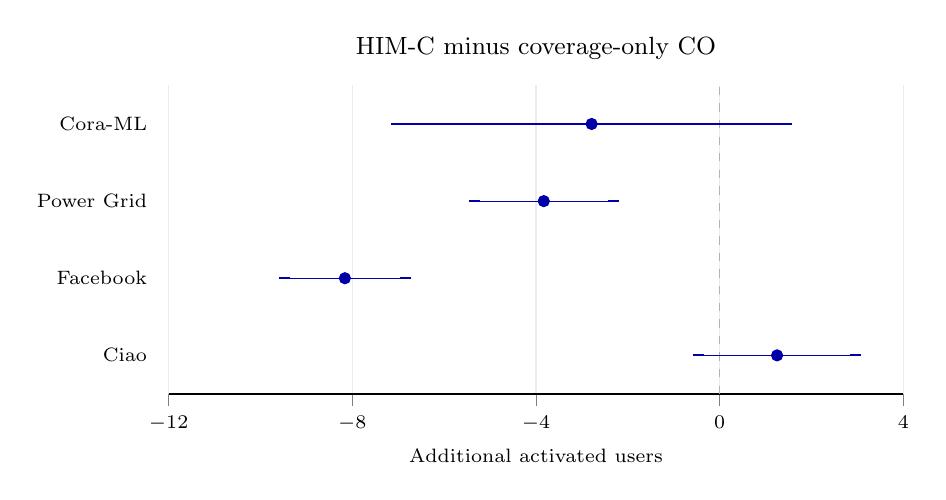
\begin{tikzpicture}\begin{axis}[
width=0.90\linewidth,height=5.5cm,title={HIM-C minus coverage-only CO},xmin=-12,xmax=4,xtick={-12,-8,-4,0,4},ymin=0.5,ymax=4.5,ytick={1,2,3,4},yticklabels={Ciao,Facebook,Power Grid,Cora-ML},xlabel={Additional activated users},axis y line*=left,y axis line style={draw=none},ytick style={draw=none},axis x line*=bottom,xmajorgrids=true,grid style={gray!15},tick align=outside,tick label style={font=\scriptsize},label style={font=\scriptsize},title style={font=\small},scale only axis=false]
\addplot[gray!60,dashed,no marks] coordinates {(0,0.5) (0,4.5)};
\addplot+[only marks,mark=*,mark size=2pt,blue!65!black,mark options={fill=blue!65!black,draw=blue!65!black},error bars/.cd,x dir=both,x explicit,error bar style={blue!65!black},error mark options={line width=0.7pt}] coordinates {
(-2.788000000,4) +- (4.239089114,0)
(-3.830000000,3) +- (1.515193683,0)
(-8.161333333,2) +- (1.322171261,0)
(1.250000000,1) +- (1.711655609,0)
};\end{axis}\end{tikzpicture}\end{minipage}

\caption{HIM-C contrasts under the same new evaluation stream. Points show mean activated-user differences and lines show unadjusted 95\% $t$ intervals across three frozen training models. Budgets are 10\% on the first three networks and approximately 5\% on Ciao. Panels use different horizontal scales; networks are not pooled. The CO comparison does not support a stable additional gain from the present HIM-prior configuration.}
\label{fig:coverage-contrasts}
\end{figure*}

\subsection{Checks, retained evidence, and practical interpretation}
The coverage audit verifies graph, probability-bank, source-result, checkpoint, selector, and simulator hashes. It reloads all 12 checkpoints, recomputes HIM-C and CO sets, and checks cardinality, bounds, outcome means, within-model paired intervals, and across-model intervals. The archived new-stream study contains 14,000 non-reused propagation simulations; repeated deterministic CO sets are evaluated once per network under that stream and reused with recorded provenance. Earlier failed or interrupted attempts are not counted as extra evidence.

Separately, the geometric implementation control forces structural blending off and recovers exactly the original ASW set on all 12 checkpoints used in the earlier ASW-J study. This checks refactoring effects on those models, not every possible input. Twenty scoped behavior/statistics tests cover the two selector extensions, tie handling, invalid inputs, budgets, isolates, and the distinction between model-level and replicate-level uncertainty.

Our main practical lesson is methodological. A representation can provide a plausible individual ranking while leaving set-level coverage poorly controlled. Modifying the selector can improve that behavior without improving the representation itself. Keeping the unsuccessful ASW-J result and the less favorable CO ablation makes the contribution inspectable: it records what was changed, what improved under fixed conditions, and which explanation the evidence does not support.


\section{Discussion and Team Integration}
\subsection{What the HIM extensions establish}
The two extensions produce different lessons. ASW-J changes a small part of the local discount rule and barely changes the final set. HIM-C replaces that local procedure with a global cumulative-coverage surrogate and changes many more seeds. Its gains on three networks support further investigation of the selection stage, not a claim that the original hyperbolic representation has been improved. The coverage-only control is essential: without it, the observed ASW-to-HIM-C gain could have been incorrectly attributed to the learned prior. Conversely, a negative or inconclusive prior ablation does not prove that learned representations are useless; the particular rank mapping and probability calibration remain part of the tested configuration.

The current evidence is conditional on one probability bank and one budget per network. Three trained models give a limited estimate of training variation. The unadjusted intervals are exploratory summaries across several comparisons, not family-wise error-controlled claims. The study also uses previously examined networks and saved encoders rather than a new held-out topology. These limits apply even where a reported interval is above zero.

\subsection{How the three methods fit together}
HIM explains how geometry supplies an individual influence prior and how a separate selector controls redundancy. DeepSN instead learns a heterogeneous propagation surrogate and allocates seeds using communities. GBIM extends the decision from users to user--information actions and optimizes expensive black-box outcomes. These are complementary stages and assumptions within influence maximization, not interchangeable implementations of one objective.

The recorded Ciao HIM-ASW and DeepSN means share the user graph, WIC bank, $k=366$, and evaluation stream 1042, but their training procedures and cascade files differ. Their numerical juxtaposition should therefore be accompanied by those design differences and the wide training intervals. The new HIM-C study uses stream 200042 and 500 simulations; its scores cannot be subtracted from DeepSN's older stream as though they were a new matched cross-method experiment. No finalized GBIM user-only equivalence result is available, so a three-method leaderboard would exceed the evidence.

\subsection{Reproducibility and division of work}
The HIM work comprises CPU environment adaptation; configurable dataset, seed, and budget entry points; checkpoint and seed-set persistence; input-aware cache keys; random-state handling; independent re-evaluation; three-network training repeats; Ciao adaptation; and the two selector extensions with controls. The other members' recorded work concerns DeepSN's native Jazz and shared-Ciao experiments and GBIM's native multiplex reproduction and adaptation. The original team milestone is retained as a dated record; its preliminary statuses are not silently converted into completed final experiments.

The retained artifacts include training commands and cache hashes, graph and probability identifiers, checkpoint hashes, exact node IDs, and per-replicate outcomes. Twenty HIM behavior/statistics tests pass. The coverage audit reloads all 12 checkpoints and reproduces both new selectors' sets before recomputing all reported means and intervals. Root-level test discovery finds no tests, so this is a scoped HIM verification claim rather than a claim about all three codebases.

\section{Conclusion}
The completed HIM component connects method reproduction to controlled improvement attempts. The author-code reproduction covers three original networks and a separate Ciao extension; it does not cover all diffusion models, budgets, large networks, or representation-learning ablations in the paper. ASW-J yields no stable gain. Global cumulative coverage yields conditional improvements over ASW on Power Grid, Facebook, and Ciao, while the coverage-only control prevents an unsupported claim about the HIM prior. This forms a concrete chain of implementation, negative evidence, redesign, and ablation. The wider team report preserves DeepSN's recorded evidence and GBIM's distinct objective boundary, leaving direct three-way ranking contingent on genuinely matched tasks and finalized result artifacts.

\appendix
\section{Artifact Index}
The report tables are generated from the archived JSON summaries, not retyped from presentation figures. Relative to the repository root, the main records are:
\begin{itemize}[leftmargin=1.2em,itemsep=0.1em]
\item \url{results/HIM/expanded_summary_2026-10-30.json}: three paper-network repetitions and five-method controls, stream 100042.
\item \url{results/HIM/structural_asw_ciao_summary_2026-10-29.json}: Ciao ASW-J and simple controls, stream 1042.
\item \url{results/HIM/coverage_summary_2026-10-30.json}: four-network HIM-C/CO study, stream 200042.
\item \url{results/HIM/coverage_verification_2026-10-30.json}: re-selection, input hashes, raw-outcome and interval checks.
\item \url{methods/HIM/CUMULATIVE_COVERAGE.md}: formulas, commands, assumptions, and attribution limits.
\end{itemize}
The seed-level JSON files named by each summary contain the complete observations. Raw data, environments, checkpoints, and caches remain local; reproducing a saved result requires the matching artifacts rather than only a textual score.

\balance
\begin{thebibliography}{99}
\bibitem{kempe} D. Kempe, J. Kleinberg, and E. Tardos, ``Maximizing the spread of influence through a social network,'' in \emph{KDD}, 2003. \href{https://doi.org/10.1145/956750.956769}{doi:10.1145/956750.956769}.
\bibitem{pastor} R. Pastor-Satorras and A. Vespignani, ``Epidemic spreading in scale-free networks,'' \emph{Phys.\ Rev.\ Lett.}, vol.~86, no.~14, pp.~3200--3203, 2001. \href{https://doi.org/10.1103/PhysRevLett.86.3200}{doi:10.1103/PhysRevLett.86.3200}.
\bibitem{him} H. Qiao et al., ``Influence strength estimation in hyperbolic space for social influence maximization,'' \emph{IEEE Transactions on Knowledge and Data Engineering}, 2026. \href{https://doi.org/10.1109/TKDE.2026.3683562}{doi:10.1109/TKDE.2026.3683562}.
\bibitem{deepsn} A. Hevapathige, Q. Wang, and A. N. Zehmakan, ``DeepSN: A sheaf neural framework for influence maximization,'' in \emph{AAAI}, 2025. \href{https://doi.org/10.1609/aaai.v39i16.33888}{doi:10.1609/aaai.v39i16.33888}.
\bibitem{hansen} J. Hansen and R. Ghrist, ``Toward a spectral theory of cellular sheaves,'' \emph{J.\ Appl.\ Comput.\ Topology}, vol.~3, pp.~315--358, 2019. \href{https://doi.org/10.1007/s41468-019-00038-7}{doi:10.1007/s41468-019-00038-7}.
\bibitem{bodnar} C. Bodnar, F. Di Giovanni, B. P. Chamberlain, P. Li{\`o}, and M. Bronstein, ``Neural sheaf diffusion: A topological perspective on heterophily and oversmoothing,'' in \emph{NeurIPS}, 2022.
\bibitem{gbim} Z. Yuan, M. Shao, and Z. Chen, ``Graph Bayesian Optimization for Multiplex Influence Maximization,'' in \emph{AAAI}, 2024. \href{https://arxiv.org/abs/2403.18866}{arXiv:2403.18866}.
\bibitem{gbimdata} GBIM authors, ``GBIM source repository and dataset instructions,'' 2024. \href{https://github.com/zirui-yuan/GBIM}{GitHub repository}.
\bibitem{ciao} J. Tang, H. Gao, H. Liu, and A. Das Sarma, ``eTrust: Understanding trust evolution in an online world,'' in \emph{KDD}, pp. 253--261, 2012; dataset source page, \href{https://www.cse.msu.edu/~tangjili/datasetcode/truststudy.htm}{Ciao and Epinions data}.
\bibitem{snapemail} J. Leskovec, K. J. Lang, A. Dasgupta, and M. W. Mahoney, ``Community structure in large networks: Natural cluster sizes and the absence of large well-defined clusters,'' Internet Mathematics, 2009; SNAP, ``Email-Eu-core temporal network,'' \href{https://snap.stanford.edu/data/email-Eu-core-temporal.html}{dataset page}.
\bibitem{deepim} C. Ling et al., ``Deep graph representation learning and optimization for influence maximization,'' in \emph{ICML}, 2023. \href{https://proceedings.mlr.press/v202/ling23b.html}{PMLR paper}.
\bibitem{poincare} M. Nickel and D. Kiela, ``Poincar\'e embeddings for learning hierarchical representations,'' in \emph{NeurIPS}, 2017. \href{https://proceedings.neurips.cc/paper/2017/hash/59dfa2df42d9e3d41f5b02bfc32229dd-Abstract.html}{Publisher paper}.
\bibitem{celf} J. Leskovec, A. Krause, C. Guestrin, C. Faloutsos, J. VanBriesen, and N. Glance, ``Cost-effective outbreak detection in networks,'' in \emph{KDD}, 2007. \href{https://las.inf.ethz.ch/files/leskovec07cost.pdf}{Author paper}.
\end{thebibliography}
\end{document}